\documentclass[11pt]{article}

\usepackage[margin=1in]{geometry}
\usepackage[utf8]{inputenc}
\usepackage[T1]{fontenc}
\usepackage{times}
\usepackage{amsmath,amssymb}
\usepackage{booktabs}
\usepackage{tabularx}
\usepackage{graphicx}
\usepackage[round]{natbib}
\usepackage{hyperref}
\usepackage{xurl}
\usepackage{xcolor}
\usepackage{enumitem}
\usepackage{microtype}
\usepackage{titling}

\setlength{\droptitle}{-1cm}
\pretitle{\begin{center}\Large\bfseries}
\posttitle{\end{center}\vspace{0.3cm}}
\hypersetup{colorlinks=true, linkcolor=black, citecolor=blue!50!black, urlcolor=blue!50!black}
\setlist{itemsep=2pt,topsep=3pt}
\newcommand{\verdict}[1]{\textsc{\MakeLowercase{#1}}}

\title{Self-Report Positions in Qwen3-1.7B Track the Input,\\ Not the Swapped-In Computation:\\ Answer-Fixed Swaps, Probes and Null Training Results}

\author{
  Sam Ramdan\\
  Independent Researcher\\
  \texttt{sr4729820@gmail.com}
}
\date{October 2026}

\begin{document}
\maketitle

\begin{abstract}
When a language model is asked about its own processing, its answer can either read the computation it has just run or work the answer out again from the question. Paper~8 of this series found evidence for the second in Qwen3-1.7B \citep{ramdan2026settling}. Here we first tried to train the first, and then probed where the information the report would need can and cannot be read. The training study and its two predecessors were preregistered; the later probe and short-training stages are exploratory.
(1)~In a two-hop question (``Which continent is the country containing \{city\} in?''), the country that later questions recover is held at the city's own tokens. Swapping the city tokens and the positions after them from a donor, from layer 11 upward, moves both the untrained self-report and a placeholder readout to the donor's country (0.840 and 0.795 of 200 held-out pairs). From layer 12 upward it moves neither (0.025). The positions after the city add no detectable country information to the readout ($+0.039$, 95\% CI $[-0.007, 0.085]$). So, in this task, reading the computation and re-reading the input cannot be told apart (preregistered verdict \verdict{SAME WINDOW}).
(2)~In two-digit multiplication, the model's confidence in its second answer digit is computed after the question and can be swapped exactly between items with the same product. Reporters trained on swapped, ordinary, injected or text-only examples all stayed at chance on 1,148 test items, with training loss at $\ln 4$ (preregistered verdict \verdict{NOT SUPPORTED}).
(3)~Linear probes trained on natural items show where the swapped-in confidence can be read. It is readable where the swap places it, at the answer digits from layer 16 (by construction): on held-out swaps whose two-way label differs, the probe agrees with the donor on 0.61--0.66. At report positions 27 and 45 tokens later, at each of the six layers probed (8 to 27), it agrees instead with the recipient's own confidence, which the question implies (donor 0.35--0.41).
(4)~Along a report placed right after the answer, the swapped-in confidence is no longer linearly readable from the very first token on. At layers 16, 20, 24 and 27, donor agreement is 0.63--0.66 at the last digit, 0.33--0.36 one token later, and 0.30--0.42 across all 27 report positions.
(5)~Short training, with two confidence levels, both report formats, and up to 900 steps of a rank-32 adapter, opened no route. Balanced accuracy on held-out swaps was 0.47--0.52 for the swap-trained reporters in the immediate format (chance 0.50). Reporters trained on ordinary labels failed too, although that label is linearly readable at the report position, so the training failure is only partly explained.
In this model, positions after the answer follow the confidence implied by the recipient's own input. The design cannot tell whether they recompute it from the question or read it from the lower, unswapped layers of the answer positions. Confidence is often taken to be the best case for direct access in humans, so the absence of a linearly readable route here is notable.
\end{abstract}

\section{Introduction}

Can a system report its own processing, or only infer it? For people, a classic answer is that many verbal reports about mental processes are inferences from implicit theories about what caused a response, rather than readouts of the process \citep{nisbett1977telling}. Theories of self-knowledge still disagree about how far that extends. On one view, access to one's own judgments and decisions is almost always interpretive \citep{carruthers2011opacity}. Confidence is the strongest case for direct access:
\begin{itemize}
\item neurons in monkey parietal cortex represent the confidence of a perceptual decision \citep{kiani2009representation};
\item microstimulating motion-sensitive neurons in visual cortex shifts confidence-based choices along with the decision, as added evidence would \citep{fetsch2014effects};
\item how well people's confidence tracks their accuracy varies with prefrontal anatomy \citep{fleming2010relating};
\item decoded neurofeedback can change reported confidence without changing performance \citep{cortese2016multivoxel}.
\end{itemize}

For language models the question has a sharper criterion. A self-report counts as introspective only if it carries information about the model's states that a third party could not read from the input \citep{song2025privileged,singh2026reality}. Paper~8 of this series tested this with interventions that keep the input's answer and the output tokens fixed \citep{ramdan2026settling}. In Qwen3-1.7B, two forced-choice self-reports did not follow an answer-position state that carried 0.90 of a logit-lens settling profile. They moved instead under swaps of the operands in the prompt (preregistered verdict \verdict{RECONSTRUCTION FROM INPUT}). This paper asks two follow-up questions.

\begin{enumerate}
\item \textbf{Can the report be trained to read the computation?} The question, and the idea of training the self-report on the model's computation rather than its input, are the author's. The specific method, proposed by the AI system that carried out this study, is to train the self-report on examples where an answer-fixed intervention has changed an internal step, so that the input cannot predict the label. It is the analogue of decoded neurofeedback, which rewards people according to states decoded from their own brain activity \citep{shibata2011perceptual,cortese2016multivoxel}. The test is whether the trained report then tracks the model's natural, unmodified computation better than any predictor that sees only the input.
\item \textbf{If it cannot, why not?} Where can the information that the report would need be read, and what does the report position carry instead?
\end{enumerate}

\paragraph{Setting and scope.} We study one model, Qwen3-1.7B \citep{yang2025qwen3}, on two tasks.
\begin{itemize}
\item \textbf{Preregistered.} The two-hop bed check (v1), its diagnosis test (v2) and the training study (v3). Decision rules were frozen with SHA-256 hashes before their data existed, and deviations were logged.
\item \textbf{Exploratory.} The probe and short-training stages (Stage~0a and Stage~0b) were run afterwards, on pilot items only, as feasibility checks for a planned fourth study. That study was stopped by its own pre-freeze rule (Section~\ref{sec:prereg}).
\end{itemize}

\paragraph{Contributions.}
\begin{itemize}
\item \textbf{A two-hop task cannot separate reading from re-reading in this model.} The country that a readout and the report recover is held at the city tokens up to layer 11, and both read it from that same window.
\item \textbf{A post-input confidence can be swapped exactly, but no reporter learns to report it.} This holds for reporters trained on interventional, observational, injected or text-only labels.
\item \textbf{Where the swapped-in value can be read.} A probe trained on natural items reads it at the answer digits, where the swap places it, and no longer reads it from the very first token after them. At every position of the immediate report, and at the final position of the delayed report, the state follows the input-implied confidence at every layer probed. Short training does not open a route, and reporters trained on ordinary labels fail as well.
\end{itemize}

\section{Related work}
\label{sec:related}

\paragraph{Criteria and untrained reports.}
\begin{itemize}
\item \textbf{The bar.} A report must beat third-party access to the input \citep{song2025privileged,singh2026reality}. Tests must also rule out causal bypassing, in which an intervention yields an accurate report without going through the state being reported \citep{morris2025bypassing}.
\item \textbf{Injected concepts.} Detection of injected concepts has been reported in large models \citep{lindsey2025emergent,macar2026mechanisms}. It can be content-agnostic \citep{lederman2026contentagnostic} or driven by a yes-bias \citep{hahami2025detecting}.
\item \textbf{Untrained reports at chance.} Across eight open models, untrained reports of injected interventions are at chance while probes read them \citep{ferrara2026owmi}.
\item \textbf{Earlier papers in this series.} An injected word reaches the answer but not the report \citep{ramdan2026injected}. Paper~8 found reconstruction from the input under answer-fixed interchange \citep{ramdan2026settling}.
\item \textbf{Our addition.} We add a localisation: where the information can be read, and what the report position carries instead.
\end{itemize}

\paragraph{Training a model to report its own states.}
\begin{itemize}
\item \textbf{Self-prediction and self-explanation.} Models have been trained to predict their own behaviour \citep{binder2024looking}, to report the attribute weights behind their own choices \citep{plunkett2025selfinterpretability}, to explain their own features and interventions \citep{li2025training,guo2026introspective}, and to report live internal signals such as routing or entropy \citep{geiping2026proprioception}.
\item \textbf{Injected states.} Supervised training on a model's own perturbed forward passes improved localisation of injected concept vectors \citep{hahami2026introspection}. Fine-tuning taught models to detect injected steering vectors \citep{fonsecarivera2026steering}. Adapters trained on labelled vectors recover multi-hop bridge entities \citep{pepper2026learning}.
\item \textbf{Interventional against output-only training.} For low-level signals such as neuron activation values, training on counterfactually perturbed values beat output-only training \citep{anon2026interventional}.
\item \textbf{Weak transfer.} External reporters given the same inputs matched self-reporters, and in-domain training gains mostly failed to transfer \citep{anon2026posthoc}. Introspection training did not transfer to a tampering probe \citep{nguyen2026prefills}. Training to disclose inserted cues transferred only weakly across cue types \citep{cheah2026faithfulness}. Models trained to predict counterfactual outcomes generalised, where interpretability techniques did not help \citep{karvonen2026counterfactual}.
\item \textbf{Non-causal channels.} Trained reporting channels can follow the prompt rather than the edited state \citep{hatua2026verbalization}. Apparent self-control can vanish once the target cannot be inferred from the prompt \citep{aoki2026neurofeedback}.
\item \textbf{Our addition.} We test interventional training of a self-report of a task-level quantity under answer-fixed swaps, comparing interventional, observational, injected and text-only labels at one budget. We then locate where the information that such training needs is readable.
\end{itemize}

\paragraph{Where intermediate results live.}
\begin{itemize}
\item \textbf{Two-hop queries.} The bridge entity is resolved in early layers, and the second hop begins only afterwards \citep{biran2024hopping}. A correct two-hop answer often comes without a decodable bridge \citep{bhan2026neurofaith}.
\item \textbf{Factual recall} is likewise localised at subject tokens \citep{meng2022locating,geva2023dissecting}.
\item \textbf{Our method.} We use answer-fixed interchange between same-answer items \citep{geiger2021inducing,zhang2023best} and probes trained on natural items. Decodable information need not be used \citep{elazar2020amnesic}, so the probes locate information but do not show its use.
\end{itemize}

\paragraph{Human metacognition.}
\begin{itemize}
\item \textbf{Confabulated reasons.} People can defend choices they did not make, with confabulated reasons \citep{johansson2005failure}.
\item \textbf{Confidence as inference.} A computational account treats confidence as a second-order inference about one's own decision, rather than a read-out of it \citep{fleming2017self}.
\item \textbf{Report training.} People have been trained, with feedback, to report naturally fluctuating EEG states \citep{frederick2012psychophysics}.
\end{itemize}

\section{Setting}
\label{sec:setting}

\paragraph{Model and interventions.}
\begin{itemize}
\item \textbf{Model.} Qwen3-1.7B has 28 blocks. It was run in bf16 with thinking off on one 8\,GB laptop GPU.
\item \textbf{Swaps.} They use paper~8's in-batch interchange. A recipient row's block outputs, at chosen positions and from a chosen layer upward, are replaced by those of a donor row computed in the same batch, so the copy is exact. ``Layer $l$'' is the output of block $l$. A swap from layer 16 therefore replaces the outputs of blocks 16--27 at the chosen positions. Later positions see the donor's states through attention from block 17 on, and the recipient's own states in blocks 0--16.
\item \textbf{Additive injections.} A unit-norm bin direction (the mean state of the items in one bin minus the mean over all items) is scaled to a multiple of the mean swap-change norm at that layer. It is applied at the same positions.
\end{itemize}

\paragraph{Self-report readout.} A forced-choice question with lettered options follows the answer. The report is the next-token letter after ``The answer is (''. The options are shown in every cyclic order, and each option's log-probability is averaged over orders, which removes letter-position bias.

\paragraph{Trained reporters.}
\begin{itemize}
\item \textbf{Adapters.} LoRA adapters on all 28 blocks, active only on the report positions. The computation being reported always runs without the adapter, so it is the unmodified model's.
\item \textbf{Arms.}
  \begin{itemize}
  \item \textbf{O:} natural labels.
  \item \textbf{I:} labels from swaps (the donor's value).
  \item \textbf{J:} labels from injected bin vectors.
  \item \textbf{X:} a reporter that reads the transcript as plain text in a fresh chat, so it sees only the input and the answer.
  \item \textbf{N:} untrained.
  \end{itemize}
\item \textbf{Budget.} Every trained arm gets the same budget.
\end{itemize}

\paragraph{Input-only bar.} P$^*$ is the best of several predictors that see only the input. It is re-chosen in every bootstrap resample, so the bar is not chosen after seeing which predictor wins.

\paragraph{Probes} (Stage~0a's method; Stage~0a was run by the coordinating session).
\begin{itemize}
\item \textbf{Classifier.} L2-regularised logistic regression on standardised block outputs, fitted with LBFGS.
\item \textbf{Regularisation.} Chosen per cell on natural rows; fixed at $\lambda = 0.5$ for the tail-position check.
\item \textbf{Folds.} Five folds grouped by product.
\item \textbf{Option order.} The report prompt is shown in one option order.
\item \textbf{B2.} A probe trained on natural rows of the training products is tested on the swapped rows of the held-out products whose label differs between donor and recipient. B2 is the share of those rows on which the probe agrees with the donor's label. With two labels, the remainder agrees with the recipient's own label.
\end{itemize}

\section{Results}

\subsection{Two-hop questions: later questions read the country from the city tokens (preregistered verdict \verdict{SAME WINDOW})}

\paragraph{Task and bed check (v1).}
\begin{itemize}
\item \textbf{Task.} ``Which continent is the country containing \{city\} in? Answer with the continent name only.'' The bridge is the country.
\item \textbf{Design.} The training study would swap region R, every position after the city name. This keeps the city, and the continent answer, fixed.
\item \textbf{Bed check.} A frozen check required a \emph{placeholder readout} to recover the country from R. In this readout, the city is replaced by a placeholder of the same token count, a run's states are copied in, and the model is asked ``Which country was the question about?'' (with a second question about the capital as a reliability check).
\item \textbf{Failure.} The check failed, so no main data were generated:
  \begin{itemize}
  \item the readout named the right country, with both readout questions agreeing, for 0.116 of 164 pilot cities whose country the model knows (threshold 0.80). Not counting disagreement as a miss, the figure is 0.354.
  \item its two questions agreed for 0.309 of 194 usable pilot cities (threshold 0.70);
  \item a swap of R from layer 0 moved the readout to the donor's country on 0.754 of reliable rows (threshold 0.90).
  \end{itemize}
\end{itemize}

\paragraph{Preregistered diagnosis (v2).}
\begin{itemize}
\item \textbf{Readout calibration} (306 held-out test cities whose country the model knows).
  \begin{itemize}
  \item Copying R at every layer gives 0.353 $[0.301, 0.408]$, against a prior of 0.314 $[0.261, 0.366]$ with nothing copied.
  \item The difference is $+0.039$ $[-0.007, 0.085]$, so an R effect of up to 0.085 is not excluded.
  \item Copying the city tokens as well gives 0.961 $[0.938, 0.980]$.
  \end{itemize}
\item \textbf{Swap boundary} (Figure~\ref{fig:window}). There are 200 pairs. Each has a recipient from the 363 usable test cities and a donor whose country the model knows, with a different country, the same continent and the same city token count. The city tokens and R are swapped from layer B upward.
  \begin{itemize}
  \item The untrained self-report (``Which country did you use to work out your answer?'') names the donor on 0.840 of rows at B~=~11, and on 0.025 at B~=~12.
  \item The placeholder readout of the swapped run gives 0.795 and 0.025.
  \item The two agree on 0.9645 of rows. The audit's pair-resampled CI is $[0.951, 0.977]$, and $\kappa = 0.741$ against 0.863, the agreement expected if each followed its own per-boundary rates independently.
  \end{itemize}
\item \textbf{R alone.} Swapping R alone at every layer, the planned training family, moves the report to the donor on 0.020 of rows. It names the recipient's own country on 0.945.
\end{itemize}
In this model, then, the country that later questions name is taken from the city-token states up to about layer 11. The self-report reads it from the same window as the readout, so this task cannot separate reading the computation from re-reading the input.

\begin{figure}[t]
\centering
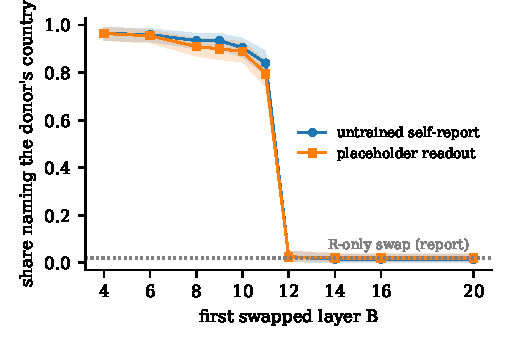
\includegraphics[width=0.55\linewidth]{fig_v2_window.pdf}
\caption{Two-hop task (v2, 200 held-out pairs, 95\% CIs). The city tokens and the positions after them are swapped from a different-country donor at layers $\ge$ B. The untrained self-report and the placeholder readout switch together between layers 11 and 12. Swapping only the positions after the city (dotted line) leaves the report on the recipient's country.}
\label{fig:window}
\end{figure}

\subsection{Multiplication confidence: exact swaps, no learnable report (preregistered verdict \verdict{NOT SUPPORTED})}

\paragraph{Replacement task.} A screen of seven candidate tasks found one whose intermediate is computed after the input (Appendix~\ref{app:search}).
\begin{itemize}
\item \textbf{Prompt.} ``What is $a$ * $b$?'', with the assistant turn prefilled to ``$a$ * $b$ = '' and the four digits teacher-forced. The items are all 3,339 pairs with $11 \le a \le b \le 99$ and a four-digit product.
\item \textbf{Quantity reported.} lp2, the model's own log-probability of its emitted second digit at the first answer-digit position. It is the computation's actual output distribution, not a lens. Its four labels are the quartiles of lp2 on training items. The cut points are $p_2 \approx 0.982$, $0.9987$ and $0.99993$, so the bins separate degrees of near-certainty.
\item \textbf{Region R.} R is the answer positions. Swapping them from layer 16 upward from a donor with the same product carried the donor's bin on all 412 different-bin test swaps, with all four digits kept.
\item \textbf{Items used.} Items were split by product. The 1,111 training and 1,148 test items that the model answers correctly are used.
\end{itemize}

\paragraph{Training and verdict.}
\begin{itemize}
\item \textbf{Training.} Each arm trained a rank-8 adapter for 300 steps of 8 examples (lr $10^{-4}$, two seeds).
\item \textbf{Gates.} All gates passed.
\item \textbf{Verdict.} \verdict{NOT SUPPORTED} (Table~\ref{tab:v3}). Arm~I did not beat the best input-only predictor on natural test items. It was not above 1/3 on two intervention families it was not trained on.
\item \textbf{Every arm at chance, X included.} The training loss of every arm fell to the label entropy within about 25 steps and stayed there (Figure~\ref{fig:training}, left). Final losses were 1.35--1.44, against $\ln 4 = 1.386$, and the trained arms' letter distributions were nearly uniform (median top-letter probability 0.26--0.31).
\item \textbf{What the verdict means.} The interventional labels gave no advantage. Because the observational and text-only arms failed too, the result does not show that observational labels do better.
\end{itemize}

\begin{table}[t]
\centering\small
\caption{v3, multiplication confidence (four bins; chance 0.25; 95\% CIs).
\textbf{T3:} natural test items (1,148). $\Delta$ is accuracy minus the best input-only predictor (the paraphrase predictor, 0.597), with that predictor re-chosen per resample.
\textbf{T1:} held-out swaps of the trained family (the label is the donor's bin).
\textbf{T2:} changed rows of two families not used to train arm~I: a single-layer swap at layer 22 (335 rows) and a bin vector at layer 18 (312 rows). The bin-vector family is arm~J's training family, applied to held-out items.
T3 accuracies are given per seed; the other accuracies are averaged over the two seeds.}
\label{tab:v3}
\setlength{\tabcolsep}{3pt}\footnotesize
\begin{tabular}{@{}lccccc@{}}
\toprule
Reporter & T3 acc. & T3 $\Delta$ & T1 different-bin & T1 same-bin & T2 pooled \\
\midrule
N, untrained & 0.272 & $-0.325$ $[-0.368, -0.281]$ & 0.277 $[0.233, 0.318]$ & 0.217 & 0.236 $[0.202, 0.272]$ \\
O, natural labels & 0.233, 0.234 & $-0.363$ $[-0.397, -0.328]$ & 0.242 $[0.210, 0.274]$ & 0.226 & 0.263 $[0.237, 0.289]$ \\
I, swap labels & 0.249, 0.229 & $-0.358$ $[-0.393, -0.322]$ & 0.301 $[0.267, 0.335]$ & 0.229 & 0.280 $[0.254, 0.306]$ \\
J, injection labels & 0.235, 0.251 & $-0.354$ $[-0.389, -0.318]$ & 0.212 $[0.181, 0.245]$ & 0.217 & 0.282 $[0.255, 0.309]$ \\
\midrule
\multicolumn{6}{@{}l}{Input-only predictors on T3: paraphrase bin 0.597; learned 0.597; external observer X 0.245; majority 0.238.} \\
\bottomrule
\end{tabular}
\end{table}

\paragraph{An exploratory signal in arm I} (found by the audit after the data were in; multiple comparisons apply). Against the level expected from its own pick frequencies (label-permutation test, 5,000 permutations), arm~I was slightly above chance on two kinds of intervened row:
\begin{itemize}
\item different-bin T1 rows: 0.301 against 0.253, $p = 0.0006$, 412 rows;
\item changed bin-vector rows: 0.322 against 0.270, $p = 0.0012$, 312 rows.
\end{itemize}

\textbf{Multiple comparisons.} Both survive a Bonferroni correction over the 20 pooled arm-by-row-set tests ($p < 0.0025$). The audit also ran 36 per-seed tests. Over all 56, only the T1 result survives.

\textbf{Per seed.} Both seeds are above their own independence level on both row sets, but each is clearly significant on only one:
\begin{itemize}
\item T1 rows: seed~1 gives 0.311 ($p = 0.0006$) and seed~0 gives 0.291 ($p = 0.11$);
\item bin-vector rows: $p = 0.0018$ for seed~0 and $p = 0.047$ for seed~1.
\end{itemize}

\textbf{Ties and size.} bf16 rounding tied the option scores of trained arms O, I and J exactly on 49--63\% of natural test rows (31\% and 63\% for the two X seeds), and ties went to the first option, which shapes their pick frequencies. The effect is not seen on same-bin swaps or untouched items, and it lies below the 1/3 that a pure tampering detector would reach. It indicates weak sensitivity to the intervention, not reading of natural confidence.

\paragraph{The confidence is largely input-determined.}
\begin{itemize}
\item On test items, lp2 and the same quantity under a paraphrased prompt have a rank correlation of 0.91.
\item A paraphrase predictor recalibrated at its own quartiles scores 0.718 (exploratory). So the bar the reporters failed to reach was, if anything, set low.
\end{itemize}

\subsection{Where the swapped-in value can be read: at the digits, not at the report (exploratory)}

The failure could mean either of two things. The information might never reach the positions where the report is computed, or it might reach them while the adapter fails to use it. Probes on the untrained model test the first.

\paragraph{Data.} The analysis used 590 natural pilot items and 474 same-product swaps from layer 16. Of these swaps, 256 change the two-way label: lp2 above or below the training median, $p_2 \approx 0.9987$. Swapped runs reproduce the donor's lp2 exactly, and all digits are kept.

\begin{itemize}
\item \textbf{At the answer digits.} Where the swap places the donor's states, the probe reads them.
  \begin{itemize}
  \item From layer 16 on, at the first digit, it agrees with the donor on 0.61--0.66 of held-out swaps. By construction, these are the donor's own states.
  \item Before the swap layer, at layers 8 and 12, it agrees with the recipient (donor 0.34--0.38).
  \item The quantity is only modestly linear even here. On all rows, the layer-27 probe reaches 0.74 with two labels and 0.43 with four. These values come from Stage~0b's extraction; Stage~0a's gives 0.74 and 0.44.
  \end{itemize}
\item \textbf{At the report positions}, at each of the six layers probed (8, 12, 16, 20, 24 and 27), the probe agrees with the donor on only 0.35--0.41 of held-out swaps, and with the recipient on the rest. This holds in all three formats:
  \begin{itemize}
  \item a turn-2 report as in v3, with v3's region R and a new user turn, but with two options in one order (Stage~0a);
  \item the same report with R restricted to the four digits, 45 tokens after them (Stage~0b);
  \item an \emph{immediate} report, appended to the answer right after its digits, 27 tokens after them (Stage~0b).
  \end{itemize}
  With four labels, both report positions sit near the majority level, and in every report cell the probe agrees more often with the recipient than with the donor.
\item \textbf{A pitfall with two labels.}
  \begin{itemize}
  \item At Stage~0a's report position, a probe trained and tested on swapped rows alone reaches 0.68--0.74, which looks like signal.
  \item But with two labels, a changed label is always the opposite of the recipient's own. A probe on the recipient's \emph{unswapped} features, given the same rows and labels, reaches 0.69--0.77.
  \item That reading therefore reflects the recipient's input-implied confidence, inverted. Only the natural-trained probe (B2) separates the two.
  \end{itemize}
\end{itemize}

\begin{figure}[t]
\centering
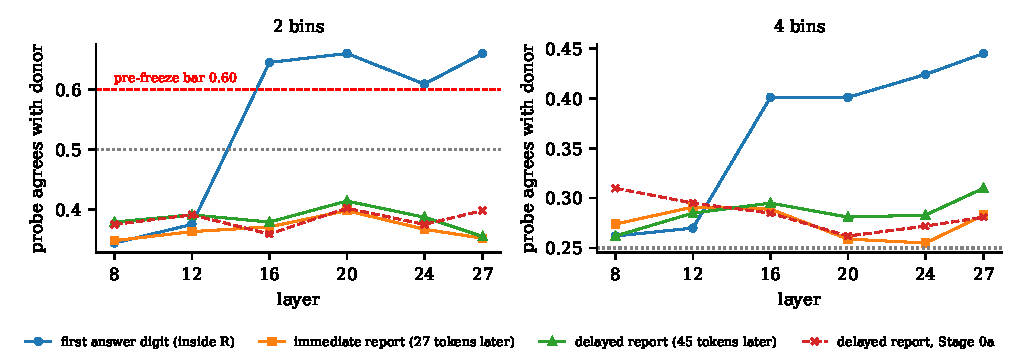
\includegraphics[width=\linewidth]{fig_probe_layers.pdf}
\caption{Where the swapped-in confidence can be linearly read (exploratory; untrained model; 256 swaps with two labels and 474 with four). Each line shows how often a probe trained on natural items agrees with the donor's label on held-out swaps where donor and recipient differ. With two labels, values below the dotted 0.5 line mean the probe follows the recipient. With four labels a probe can agree with neither; at the report positions it agrees more often with the recipient than with the donor in every cell (not plotted). Red dashed line: the 0.60 bar fixed by the coordinating session before the planned v4 freeze.}
\label{fig:probes}
\end{figure}

\subsection{The swapped-in value is no longer linearly readable from the first token after the digits (exploratory)}

To see how far the swapped-in confidence travels, the same probe method was applied to the last answer digit and to each of the 27 positions of the immediate report (Figure~\ref{fig:tailpos}). It used the same 256 swaps, layers 12, 16, 20, 24 and 27, and regularisation fixed at $\lambda = 0.5$.
\begin{itemize}
\item \textbf{The last digit} is inside the swapped region. At layers 16, 20, 24 and 27, the probe follows the donor there (0.63--0.66). At layer 12, before the swap, it follows the recipient (0.36).
\item \textbf{The first token after the digits} already follows the recipient: donor agreement is 0.33--0.36 at layers 16, 20, 24 and 27. Over the first three positions it is at most 0.39, and over all 27 positions of the immediate report it is 0.30--0.42.
\item \textbf{Where the donor's states are visible.} From block 17 on, the positions after the digits attend to the donor's digit states. Even so, their own states follow the recipient at every layer probed.
\end{itemize}
So no position of the immediate report carries the swapped-in value in a linearly readable form. A trained route would probably have to be built rather than tapped.

\begin{figure}[t]
\centering
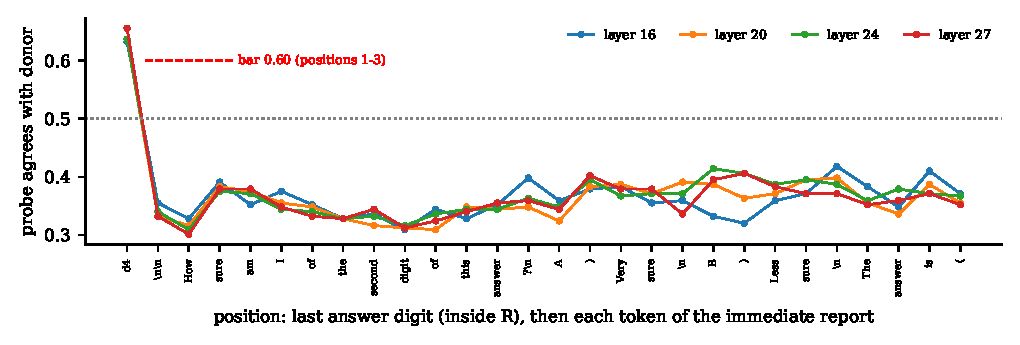
\includegraphics[width=\linewidth]{fig_tailpos.pdf}
\caption{How far the swapped-in confidence travels (exploratory; untrained model; 256 swaps whose two-way label differs; layers 16, 20, 24 and 27, with layer 12 omitted). The probe is trained on natural items. It follows the donor at the last answer digit, which is inside the swapped region, and follows the recipient from the very first token after it, through the whole immediate report. Red dashed segment: the 0.60 bar for the first three positions after the digits, set by the coordinating session before the result.}
\label{fig:tailpos}
\end{figure}

\subsection{Short training opens no route, and ordinary labels fail too (exploratory)}

The probes show that the untrained report positions do not carry the swapped-in state in a linearly readable form. A trained adapter might still learn to attend back to it. We trained small reporters on pilot items, 190 for training and 124 held out, with disjoint products (Table~\ref{tab:s0b}).
\begin{itemize}
\item \textbf{Arm~I.} Rank 8 at learning rates $10^{-4}$ and $10^{-3}$ for up to 300 steps, in both formats. Rank 32 at $3 \times 10^{-4}$ for up to 900 steps, immediate format only.
\item \textbf{Arm~O, immediate format.} Rank 8 at $10^{-3}$ for up to 300 steps, and rank 32 at $3 \times 10^{-4}$ for up to 900 steps.
\item \textbf{Result.} No reporter learned.
  \begin{itemize}
  \item Twelve of the 16 checkpoints answered almost constantly, giving the same answer on at least 87\% of natural items; the other four answered ``Very sure'' on 31--67\% of natural items, with natural accuracy 0.45--0.53.
  \item Training loss settled near $\ln 2$ within 50--150 steps (Figure~\ref{fig:training}, right).
  \item Balanced accuracy on held-out swaps was 0.47--0.52 for arm~I in the immediate format, and 0.46--0.52 over all runs (chance 0.50).
  \end{itemize}
\item \textbf{Arm~O against the question.}
  \begin{itemize}
  \item Arm~O's accuracy on natural items peaked at 0.573, the majority answer.
  \item Predictors that see only the question reach 0.895 on the same items. At the report positions, the recipient's own label is linearly readable from its unswapped state: 0.67--0.72 at the immediate report, the format arm~O was trained on, and 0.69--0.77 at Stage~0a's delayed report.
  \item So O's failure is not explained by missing information. At these budgets, and in this format, the adapters did not learn even a readable, input-implied label.
  \end{itemize}
\item \textbf{The untrained immediate report} was below chance on natural items (0.347). It answered ``Very sure'' on 47 of 71 ``Less sure'' items, and on 19 of 53 ``Very sure'' items.
\end{itemize}
The largest budget tried was rank 32 for 900 steps of 8 examples.

\begin{table}[t]
\centering\small
\caption{Short training with two labels (exploratory; pilot items; one seed).
\textbf{Balanced:} mean accuracy over different-label and same-label held-out swaps (24 and 62 rows; chance 0.50).
\textbf{Natural:} held-out natural items (124; majority 0.573, question-only predictors 0.895).
\textbf{``Very sure'' share:} the share of natural items answered ``Very sure'', with scores averaged over both option orders. Values near 0 or 1 mean a constant answer.}
\label{tab:s0b}
\setlength{\tabcolsep}{4pt}\footnotesize
\resizebox{\linewidth}{!}{%
\begin{tabular}{@{}lccccc@{}}
\toprule
Run & Steps & Balanced & Natural & ``Very sure'' share & Final loss \\
\midrule
untrained, immediate / delayed & 0 & 0.506 / 0.487 & 0.347 / 0.419 & 0.53 / 0.96 & -- \\
I, immediate, rank 8, lr $10^{-3}$ & 150 / 300 & 0.510 / 0.501 & 0.556 / 0.452 & 0.03 / 0.93 & 0.665 / 0.707 \\
I, immediate, rank 8, lr $10^{-4}$ & 150 / 300 & 0.518 / 0.474 & 0.573 / 0.427 & 0.00 / 0.97 & 0.623 / 0.699 \\
I, delayed, rank 8, lr $10^{-3}$ & 150 / 300 & 0.463 / 0.498 & 0.532 / 0.435 & 0.43 / 0.88 & 0.683 / 0.781 \\
I, delayed, rank 8, lr $10^{-4}$ & 150 / 300 & 0.518 / 0.482 & 0.573 / 0.427 & 0.00 / 1.00 & 0.649 / 0.697 \\
O, immediate, rank 8, lr $10^{-3}$ & 150 / 300 & 0.462 / 0.518 & 0.516 / 0.573 & 0.31 / 0.00 & 0.580 / 0.735 \\
I, immediate, rank 32, lr $3\times10^{-4}$ & 300 / 600 / 900 & 0.501 / 0.489 / 0.469 & 0.460 / 0.452 / 0.419 & 0.90 / 0.67 / 0.99 & 0.764 / 0.723 / 0.669 \\
O, immediate, rank 32, lr $3\times10^{-4}$ & 300 / 600 / 900 & 0.518 / 0.518 / 0.476 & 0.573 / 0.573 / 0.500 & 0.00 / 0.00 / 0.57 & 0.740 / 0.694 / 0.700 \\
\bottomrule
\end{tabular}}
\end{table}

\begin{figure}[t]
\centering
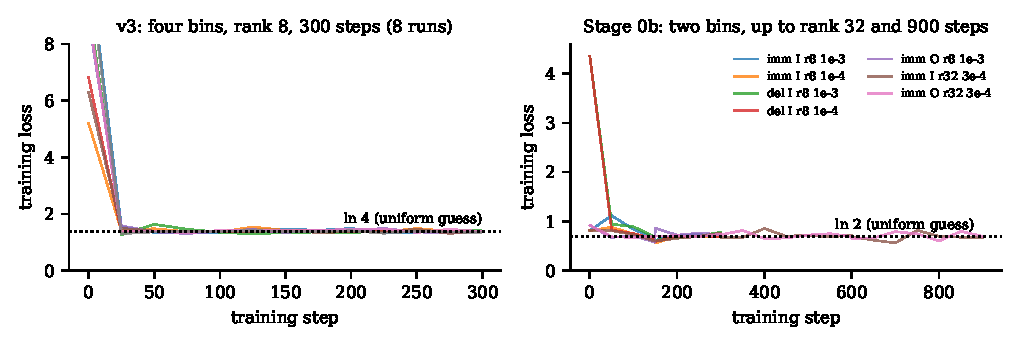
\includegraphics[width=\linewidth]{fig_training.pdf}
\caption{Training losses. Left: v3, four labels, rank 8, 300 steps, eight runs (four arms, two seeds); every run settles at the label entropy ($\ln 4$). Right: Stage~0b, two labels, rank 8 or 32, up to 900 steps; every run settles near $\ln 2$.}
\label{fig:training}
\end{figure}

\section{Discussion}

\paragraph{What the report positions carry.} The two tasks give different kinds of evidence.
\begin{itemize}
\item \textbf{Two-hop questions.} Reading the computation and re-reading the input could not be told apart, because the country the reports name is read from the input tokens.
\item \textbf{Multiplication.} Here the swap separates what the input implies from the part of the computation that set the output. The report positions carried, in linearly readable form, the confidence that the recipient's own input implies, not the swapped-in confidence that determined the model's actual output. This held at every layer probed, whether the question came 27 or 45 tokens after the answer.
\item \textbf{Relation to earlier results.} This is consistent with paper~8's \verdict{RECONSTRUCTION FROM INPUT}, now at the level of the report position's internal state, for a naturally occurring quantity whose input and answer are held fixed. It matches the injection literature \citep{ferrara2026owmi,hatua2026verbalization}.
\item \textbf{Two routes remain open.} The positions may recompute the confidence from the question, or read it from the lower layers of the answer positions, which the swap leaves untouched.
\end{itemize}

\paragraph{Why training does not find a route} (interpretation, not tested).
\begin{itemize}
\item \textbf{The swap labels need a route the untrained model lacks.} The swapped-in value is not linearly readable at any position probed after the digits: every position of the immediate report, and the final position of the delayed report.
\item \textbf{The ordinary labels need no such route, and their failure is unexplained.} A question-only predictor reaches 0.895 on Stage~0b's 124 held-out items (0.867 on the 1,148 v3 test items with two labels), and the input-implied label is linearly readable at the report position. Yet arm~O stayed at the majority answer. The loss, the letter format or the budget may be responsible.
\item \textbf{The labels are fine-grained.} They separate degrees of near-certainty, and even at the digits the quantity is only modestly linear (0.74).
\item \textbf{A pre-check for future work.} Before training on interventional labels, probe the report position and the positions just after the answer, as here.
\end{itemize}

\paragraph{Relation to human introspection.}
\begin{itemize}
\item \textbf{The inference view.} The result is consistent with it: the report positions carry what the question implies, not the swapped-in part of the process \citep{nisbett1977telling,carruthers2011opacity}. The design cannot rule out that they read the unswapped lower layers of the answer positions instead.
\item \textbf{Confidence is the hard case for that view.} In monkeys, parietal neurons represent it \citep{kiani2009representation}, and adding sensory evidence by microstimulation moves confidence-based choices \citep{fetsch2014effects}. In humans, how well it tracks accuracy varies with brain structure \citep{fleming2010relating}, and decoded neurofeedback can move it \citep{cortese2016multivoxel}.
\item \textbf{What the model lacks.} In Qwen3-1.7B, when a swap changes the confidence at the answer positions, the change is not linearly detectable at the positions that report it. They carry the confidence the question implies instead.
\item \textbf{What this does not show.} It does not show that language models cannot have such a route. It shows no linearly detectable route in an untrained 1.7B model, and that small adapters did not build one.
\end{itemize}

\paragraph{Limitations.}
\begin{itemize}
\item \textbf{Scope.} One model at 1.7B, two tasks, and forced-letter reports.
\item \textbf{Swap depth.} The swap starts at layer 16, so later positions still see the recipient's own answer-position states in blocks 0--16. ``Recomputes from the question'' and ``reads earlier layers of the answer positions'' are not separated.
\item \textbf{Linear probes.} A nonlinear readout might find information that a linear probe misses, although the trained adapters did not. The probes used one option order, six layers (five in the tail check), and only the final position of the delayed report.
\item \textbf{Small training budgets.} The largest was rank 32 for 900 steps on 190 pilot items (Stage~0b), or rank 8 for 300 steps (v3). The planned ladder, up to 3,000 steps, was not run. Ordinary labels failed as well, so the budgets may simply have been too small.
\item \textbf{A metacognitive quantity.} The multiplication intermediate is the model's confidence, not an intermediate value of the task, and its labels separate degrees of near-certainty.
\item \textbf{Exploratory stages.} The probe and short-training stages are exploratory, on pilot items, with small held-out sets (24 different-label swaps in Stage~0b).
\item \textbf{The two-label probe artefact} is explained above; only probes trained on natural rows are interpretable.
\item \textbf{The v3 arm-I signal} was found after the data were in, and is reported with its multiple-comparison caveat.
\end{itemize}

\section{Preregistration, deviations and reproducibility}
\label{sec:prereg}

\paragraph{Freezes.} Three studies were frozen with SHA-256 hashes of their preregistration and code, including the imported modules, before their data existed:
\begin{itemize}
\item v1, the two-hop training study, stopped at its bed check;
\item v2, the diagnosis test;
\item v3, the multiplication training study.
\end{itemize}
A pre-data fix to v3's code-test mode was logged with an amendment hash. One hashed file no longer matches: the study's \texttt{README.md}, a file index with no decision rule, which was extended after the v1 freeze without a log entry at the time (logged in \texttt{DEVIATIONS.md}, 2026-10-25). Every other hashed file matches.

\paragraph{The planned fourth study (v4).}
\begin{itemize}
\item \textbf{Design.} Two labels, a budget ladder, a learnability gate, and an immediate report as the primary format. It was drafted but not frozen.
\item \textbf{The stopping rules.} The coordinating session set them. It told the author about the first after sending it, and the author approved the plan that included the second without being shown its threshold. The first required, before the freeze, that a natural-trained probe agree with the donor above 0.60 at the new report position; the ladder would not run otherwise. The second, received before the tail-position check ran, allowed a one-token report tag to be proposed only if that agreement exceeded 0.60 at one of the first three positions after the digits.
\item \textbf{The outcome.} Stage~0b found 0.35--0.40 at the immediate report position and at most 0.39 at the first three positions. So v4 was stopped, and no v4 ladder or main data exist.
\end{itemize}

\paragraph{Deviations and audits.}
\begin{itemize}
\item \textbf{Deviation log.} Every change is logged in \texttt{DEVIATIONS.md}, including an overnight laptop suspension during v3's main run that did not affect its data.
\item \textbf{Audits.} Independent audits recomputed the v1--v3 results and every number in this manuscript. The reports are in \texttt{audit/}.
\item \textbf{How the numbers were produced.} Each number in this manuscript was typed in from the file \texttt{numbers.json}, which \texttt{paper/make\_numbers.py} generates from the result files, or from the files named in the text. The manuscript audit checks each against the raw files.
\end{itemize}

\paragraph{Files.} The study folder holds the preregistrations, code, deviation logs, per-item results and audits. They are released in the repository (\url{https://github.com/Somebodyhere101/self-report-tracks-input}). The eight result files larger than 2\,MB (\texttt{res\_v2/premise.json} and the seven \texttt{res\_v3/eval\_*.json}) are only in the Zenodo record linked from the repository, which also archives the whole repository. Model weights, the probes' stored hidden-state features, job logs and the lab's GPU-lock wrapper are withheld, and the model's free-text answers in the item screens were removed; the repository's \texttt{DATA.md} lists each and how to rebuild it.

\appendix
\section{Replacement-task search}
\label{app:search}
Each of seven candidates was screened on 6--48 items against v1's checks:
\begin{itemize}
\item the task is answered correctly;
\item there is a causal ground truth that readouts agree on;
\item an answer-fixed swap moves it.
\end{itemize}

The six candidates not used:
\begin{itemize}
\item \textbf{Parity of a single-digit sum:} the model answered ``Even'' to everything.
\item \textbf{A sum compared with a threshold:} the model always answered ``Yes''.
\item \textbf{Digits of a sum:} the model copied an operand digit.
\item \textbf{The carry in a written sum:} the sums were right, but the carry question failed even with the operands visible.
\item \textbf{A product's least-sure digit:} the label was degenerate, always the second digit.
\item \textbf{A sum above or below 50:} borderline, so not pursued.
\end{itemize}

The seventh, confidence in a product's second digit, passed:
\begin{itemize}
\item answers correct on 41/48;
\item probability and entropy labels agreeing on 47/48;
\item same-product swaps moving the label on 10/10.
\end{itemize}

The logs are in \texttt{diag/}. For candidates 3--7 they are deterministic CPU reruns made on 2026-10-22, each labelled as such.

\section*{AI use and author contribution}

This study was carried out by an AI system: Claude (Anthropic), Claude Opus 5.5 (\texttt{claude-opus-5-5}), in every session, including the audit and reviewer sessions. It ran as Claude Code agent sessions on the author's computer, and it:
\begin{itemize}
\item checked the novelty of the idea;
\item chose the design of every stage and wrote each preregistration;
\item wrote all the code;
\item ran every experiment on the author's hardware;
\item analysed the results;
\item searched for and checked the cited literature;
\item wrote this manuscript.
\end{itemize}
One Claude session coordinated the others and passed on the author's requests. On the author's behalf, after the author approved a fourth study and asked for a quick small-scale check of whether it could work, it made that study's design decisions, ran Stage~0a, and set the pre-freeze rules that stopped it.

The study's question, whether a model's self-report can be trained to read its own computation rather than reconstruct it from the input, and the suggestion to answer it by training, were the author's. A related item, a trained self-report on a looped model's depth, was already on a shortlist that the AI system had produced and shown to the author the day before. The AI system proposed the method in reply: training the self-report on examples where an answer-fixed intervention changed an internal step, and testing it against the model's natural computation and an input-only predictor. It also proposed decoded neurofeedback as the human analogue, in reply to the author's question about whether people can do this. The replacement task, the probe stages and the stopping rules were the AI system's. The author started the study, asked for it to be finished overnight, approved the fourth study and its feasibility stage, and approved drafting this paper; the second study ran under the first study's frozen rules without a separate approval. The author provided the computing hardware and decided to release the study. The author did not independently check the code, analyses or technical claims.

\paragraph{How the work was checked.} Independent Claude sessions acting as auditors recomputed the results from the raw files. One audit covered v1 and v2, one covered v3, and one covered every number in this manuscript. Their reports are in \texttt{audit/}.

\bibliographystyle{plainnat}
\bibliography{references}

\end{document}
